% cd /storage/emulated/0/Documents/documents/latex/1920/Grade-8/2nd/domain-and-range-of-a-function/&& pdflatex hand-domain-and-range-of-a-function.tex && divide 1x2 hand-domain-and-range-of-a-function.pdf


\documentclass[handout]{beamer} 

\usepackage{pgfpages} 
\mode<handout>{%
\pgfpagesuselayout{4 on 1}[%letterpaper, 
legalpaper,% landscape, 
border shrink=1mm] 
}

\usepackage{xcolor}
\usepackage{anyfontsize}
\usepackage{enumitem}
\usepackage{multicol}
\usepackage{amsmath, makecell}
\usepackage{tabularx} 
\usepackage{gensymb}
\usepackage{wasysym} %for checked symbol 
\usepackage{multirow}
\usepackage{graphicx, tipa}
\usepackage{tikz}
\usetikzlibrary{angles,quotes}
\usepackage{pgfplots} 
\usetikzlibrary{calc}
\pgfplotsset{compat=newest}
\usetikzlibrary{arrows.meta}
\usetikzlibrary{intersections}
\usetikzlibrary{decorations.pathreplacing}
\usepackage{flafter}
%\usepackage{fourier} 
\usepackage{amsmath,amssymb,cancel,units}
\usepackage{microtype} % nicer output 
\usepackage{hfoldsty} % nicer output 
\usepackage{fixltx2e} 
\usepackage{mathptmx}
\usepackage{numprint}
\usepackage[T1]{fontenc}
\usepackage[utf8]{inputenc} 
\usepackage{stackengine} %to define \pesos 
\usepackage{lmodern} %scalable font
\usepackage{booktabs}
\usepackage{array}


\pagenumbering{gobble}
%\linespread{0.9}
\newcommand{\vspce}{\vspace{0.75ex}}

\newcommand{\hspce}{\hspace{0.5em}}

\newcommand{\blank}{\underline{\hspace{2em}}}%{\rule{1em}{0.15ex}}

\newcommand{\arc}[1]{{% 
\setbox9=\hbox{#1}% 
\ooalign{\resizebox{\wd9}{\height}{\texttoptiebar{\phantom{A}}}\cr#1}}}


\newcommand\pesos{\stackengine{-1.4ex}{P}{\stackengine{-1.25ex}{$-$}{$-$}{O}{c}{F}{F}{S}}{O}{c}{F}{T}{S}} 


\renewcommand\theadalign{bc} 

\renewcommand\theadfont{\bfseries} 

\renewcommand\theadgape{\Gape[4pt]} 

\renewcommand\cellgape{\Gape[4pt]} 

\pagenumbering{gobble}

\newcolumntype{Y}{>{\centering\arraybackslash}X} %for tabularx

\newcolumntype{R}{>{\raggedleft\arraybackslash}X} %for tabularx

\newcolumntype{Z}{>{\raggedleft\arraybackslash}X} %for tabularx

\newcolumntype{L}{>{\raggedright\arraybackslash}X} %for tabularx

\newcolumntype{A}[1]{>{\raggedright\arraybackslash}p{#1}} %for longtable LEFT

\newcolumntype{C}[1]{>{\centering\arraybackslash}p{#1}} %for longtable CENTER

\newcolumntype{B}[1]{>{\raggedleft\arraybackslash}p{#1}} %for longtable RIGHT 
 
\renewcommand{\tabularxcolumn}[1]{>{\small}m{#1}}

\newcolumntype{N}[1]{>{\raggedleft}p{#1}} %for tabular left 

\newcolumntype{M}[1]{>{\raggedright\arraybackslash}p{#1}} %for tabular right 

\newcommand{\myaxis}{xticklabels={}, 
yticklabels={}, 
ymin=-10, ymax=10,
xmin=-10, xmax=10,
axis lines = center, 
inner axis line style={Latex-Latex,very thick}, 
grid=both,
minor tick num=4, 
tick align=inside} % grid without labels, origin at the center, 10 units from origin

\newcommand{\axisfive}{xticklabels={}, 
yticklabels={}, 
ymin=-5, ymax=5,
xmin=-5, xmax=5,
axis lines = center, 
inner axis line style={Latex-Latex,very thick}, 
grid=both,
minor tick num=1, 
tick align=inside} % grid with labels, origin at the center, 5 units from origin 

\newcommand \redcheck {{\color{red}\checkmark}}



%\newcommand{\vertadjust}{\vspace*{-1.5in}} % for letterpaper
%\newcommand{\vertadjustb}{\vspace*{-1.5in}} % for letterpaper
\newcommand{\vertadjust}{\vspace*{-2.5in}} % for legalpaper
\newcommand{\vertadjustb}{\vspace*{-2.5in}} % for legalpaper

\def\gridscale{0.4}


\begin{document} 

% frame 1
\vertadjust
\begin{frame} 
\begin{center}
\textbf{Domain and Range of a Function}
\end{center}

\vspace*{1ex}

Domain: the set of all permissible values of $x$ that  give real values  for  $y$ 
 
\vspce 

Range: the set of permissible  values  for ${y }$   or  ${f(x) }$  that give the values of  ${x }$   real numbers

\vspce 

Asymptote: a line that the graph of a function approaches but never intersects

 %\\
%\input{hand-domain-and-range-of-a-function-input1}
\def\figdir{/storage/emulated/0/Documents/documents/latex/1920/Grade-8/2nd/domain-and-range-of-a-function/f}

\textbf{Practice Exercises}

\vspce

A. Determine the domain and the range of each graph.
\begin{enumerate}[label = \arabic*. ]
\begin{multicols}{2}
%1
\item 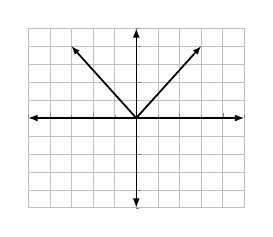
\begin{tikzpicture}[scale=\gridscale]
\begin{axis}[\axisfive]

\draw[->, >=latex, ultra thick] (0,0) -- (-3,4);
\draw[->, >=latex, ultra thick] (0,0) -- (3,4);

\end{axis} 
\end{tikzpicture}  
%2
\item 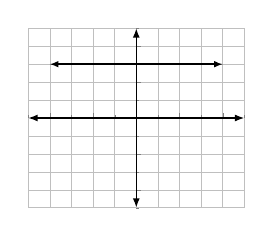
\begin{tikzpicture}[scale=\gridscale]
\begin{axis}[\axisfive]

\draw[<->, >=latex, ultra thick] (-4,3) -- (4,3);

\end{axis} 
\end{tikzpicture}  
%3
\item 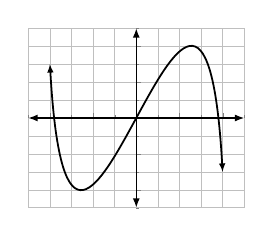
\begin{tikzpicture}[scale=\gridscale]
\begin{axis}[\axisfive]

\draw[<->, >=latex, ultra thick](-4,3)..controls(-3,-18) and (3,18)..(4,-3);

\end{axis} 
\end{tikzpicture}  
%4
\item 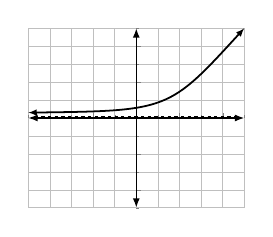
\begin{tikzpicture}[scale=\gridscale]
\begin{axis}[\axisfive]

\draw[<->, >=latex, ultra thick](-5,0.3)..controls(1.5,0.4) ..(5,5);
\draw[thin, dashed](-4.7,0.1)--(4.7,0.1); 

\end{axis} 
\end{tikzpicture}  
%5 
\item 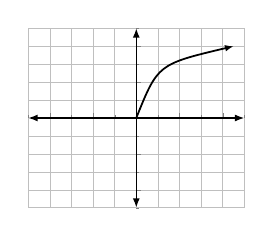
\begin{tikzpicture}[scale=\gridscale]
\begin{axis}[\axisfive]

\draw[->, >=latex, ultra thick](0,0.)..controls(1,3) ..(4.5,4);

\end{axis} 
\end{tikzpicture}  
%6
\item 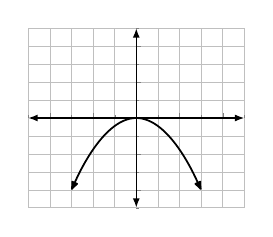
\begin{tikzpicture}[scale=\gridscale]
\begin{axis}[\axisfive]

\draw[<->, >={Latex[round]},  ultra thick] (-3,-4) parabola bend (0,0) (3,-4);

\end{axis} 
\end{tikzpicture}  
\end{multicols} 
\end{enumerate}  
B. Find the domain of each function.
\begin{enumerate}[label = \arabic*. ]
\item \hspce ${g(x)  = 5x+1 }$ 
\vspce 
\item \hspce ${g(x)  =  \sqrt{x} }$ 
\vspce 
\item \hspce ${ g(x) = \displaystyle  \frac{x+4}{x-2} }$ 
\vspce 
\item \hspce ${ g(x)  =  \sqrt{ x-8}}$ 
\vspce 
\item \hspce ${g(x)  =  \displaystyle  \frac{3x}{x+6}}$ 
\end{enumerate}  
%\def\figdir{/storage/emulated/0/Documents/documents/latex/1920/Grade-8/2nd/domain-and-range-of-a-function/f}

\textbf{Problem Set}

\vspce

A. Determine the domain and the range of each graph.
\begin{enumerate}[label = \arabic*. ]
\begin{multicols}{2}
%1
\item 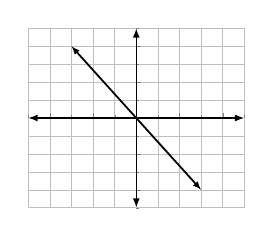
\begin{tikzpicture}[scale=\gridscale]
\begin{axis}[\axisfive]

\draw[<->, >=latex, ultra thick] (-3,4) -- (3,-4);

\end{axis} 
\end{tikzpicture}  
%2
\item 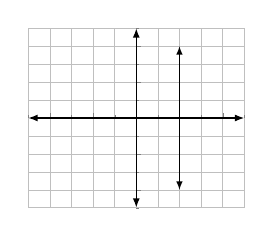
\begin{tikzpicture}[scale=\gridscale]
\begin{axis}[\axisfive]

\draw[<->, >=latex, ultra thick] (2,4) -- (2,-4);

\end{axis} 
\end{tikzpicture}  
%3
\item 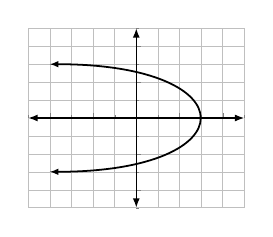
\begin{tikzpicture}[scale=\gridscale]
\begin{axis}[\axisfive]

\draw[<->, >=latex, ultra thick](-4,3)..controls(5.2,3) and (5.2,-3)..(-4,-3);

\end{axis} 
\end{tikzpicture}  
%4
\item 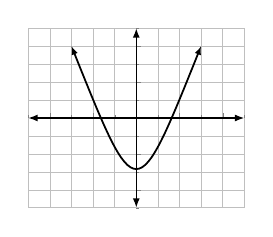
\begin{tikzpicture}[scale=\gridscale]
\begin{axis}[\axisfive]

\draw[<->, >=latex, ultra thick](-3,4)..controls(0,-5)..(3,4);

\end{axis} 
\end{tikzpicture}  
%5 
\item 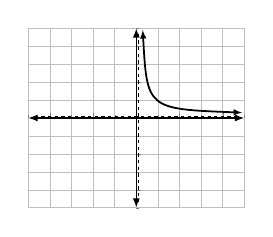
\begin{tikzpicture}[scale=\gridscale]
\begin{axis}[\axisfive]

\draw[<->, >=latex, ultra thick](0.3,4.9)..controls(0.5,0.5) ..(4.9,0.3);
\draw[thin, dashed](-4.7,0.1)--(4.7,0.1);
\draw[thin, dashed](0.1,4.7)--(0.1,-4.7); 

\end{axis} 
\end{tikzpicture}  
%6
\item \input{\figdir/fig-domain-and-range-of-a-function-b6} 
\end{multicols} 
\end{enumerate}  

B. Find the domain of each function.
\begin{enumerate}[label = \arabic*. ]
\item \hspce ${g(x)  = x-7 }$ 
\vspce 
\item \hspce ${g(x)  =  \sqrt{x+1} }$ 
\vspce 
\item \hspce ${ g(x) = \displaystyle  \frac{3x+4}{x-1} }$ 
\vspce 
\item \hspce ${ g(x)  =  \sqrt{ 2x-4} }$ 
\vspce 
\item \hspce ${g(x)  = \displaystyle  \frac{x+4}{3x-5} }$ 
\end{enumerate}  

\end{frame}

% frame 2
\vertadjust
\begin{frame} 
%\begin{center}
\textbf{Domain and Range of a Function}
\end{center}

\vspace*{1ex}

Domain: the set of all permissible values of $x$ that  give real values  for  $y$ 
 
\vspce 

Range: the set of permissible  values  for ${y }$   or  ${f(x) }$  that give the values of  ${x }$   real numbers

\vspce 

Asymptote: a line that the graph of a function approaches but never intersects

% \\
%\def\figdir{/storage/emulated/0/Documents/documents/latex/1920/Grade-8/2nd/domain-and-range-of-a-function/f}

\textbf{Practice Exercises}

\vspce

A. Determine the domain and the range of each graph.
\begin{enumerate}[label = \arabic*. ]
\begin{multicols}{2}
%1
\item 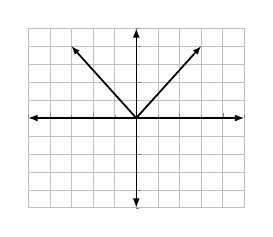
\begin{tikzpicture}[scale=\gridscale]
\begin{axis}[\axisfive]

\draw[->, >=latex, ultra thick] (0,0) -- (-3,4);
\draw[->, >=latex, ultra thick] (0,0) -- (3,4);

\end{axis} 
\end{tikzpicture}  
%2
\item 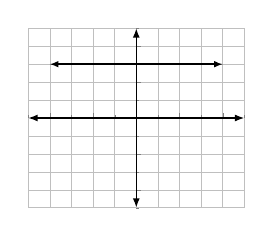
\begin{tikzpicture}[scale=\gridscale]
\begin{axis}[\axisfive]

\draw[<->, >=latex, ultra thick] (-4,3) -- (4,3);

\end{axis} 
\end{tikzpicture}  
%3
\item 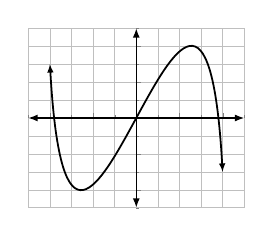
\begin{tikzpicture}[scale=\gridscale]
\begin{axis}[\axisfive]

\draw[<->, >=latex, ultra thick](-4,3)..controls(-3,-18) and (3,18)..(4,-3);

\end{axis} 
\end{tikzpicture}  
%4
\item 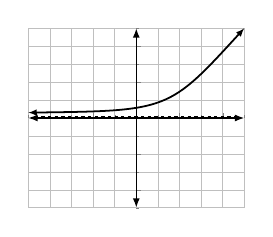
\begin{tikzpicture}[scale=\gridscale]
\begin{axis}[\axisfive]

\draw[<->, >=latex, ultra thick](-5,0.3)..controls(1.5,0.4) ..(5,5);
\draw[thin, dashed](-4.7,0.1)--(4.7,0.1); 

\end{axis} 
\end{tikzpicture}  
%5 
\item 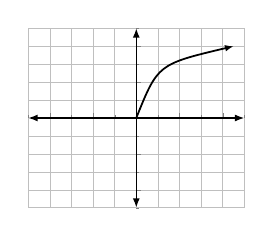
\begin{tikzpicture}[scale=\gridscale]
\begin{axis}[\axisfive]

\draw[->, >=latex, ultra thick](0,0.)..controls(1,3) ..(4.5,4);

\end{axis} 
\end{tikzpicture}  
%6
\item 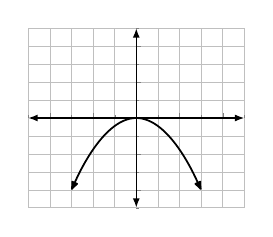
\begin{tikzpicture}[scale=\gridscale]
\begin{axis}[\axisfive]

\draw[<->, >={Latex[round]},  ultra thick] (-3,-4) parabola bend (0,0) (3,-4);

\end{axis} 
\end{tikzpicture}  
\end{multicols} 
\end{enumerate}  
%B. Find the domain of each function.
\begin{enumerate}[label = \arabic*. ]
\item \hspce ${g(x)  = 5x+1 }$ 
\vspce 
\item \hspce ${g(x)  =  \sqrt{x} }$ 
\vspce 
\item \hspce ${ g(x) = \displaystyle  \frac{x+4}{x-2} }$ 
\vspce 
\item \hspce ${ g(x)  =  \sqrt{ x-8}}$ 
\vspce 
\item \hspce ${g(x)  =  \displaystyle  \frac{3x}{x+6}}$ 
\end{enumerate}  
%\input{hand-domain-and-range-of-a-function-input2}
\vspace*{1ex}
\def\figdir{/storage/emulated/0/Documents/documents/latex/1920/Grade-8/2nd/domain-and-range-of-a-function/f}

\textbf{Problem Set}

\vspce

A. Determine the domain and the range of each graph.
\begin{enumerate}[label = \arabic*. ]
\begin{multicols}{2}
%1
\item 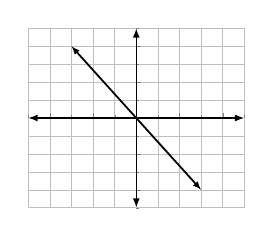
\begin{tikzpicture}[scale=\gridscale]
\begin{axis}[\axisfive]

\draw[<->, >=latex, ultra thick] (-3,4) -- (3,-4);

\end{axis} 
\end{tikzpicture}  
%2
\item 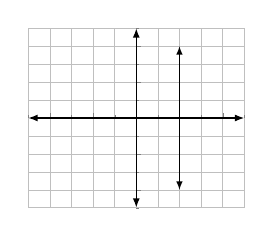
\begin{tikzpicture}[scale=\gridscale]
\begin{axis}[\axisfive]

\draw[<->, >=latex, ultra thick] (2,4) -- (2,-4);

\end{axis} 
\end{tikzpicture}  
%3
\item 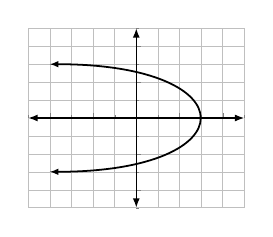
\begin{tikzpicture}[scale=\gridscale]
\begin{axis}[\axisfive]

\draw[<->, >=latex, ultra thick](-4,3)..controls(5.2,3) and (5.2,-3)..(-4,-3);

\end{axis} 
\end{tikzpicture}  
%4
\item 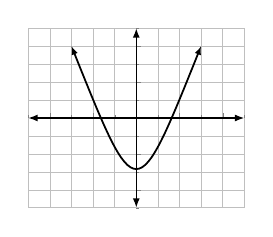
\begin{tikzpicture}[scale=\gridscale]
\begin{axis}[\axisfive]

\draw[<->, >=latex, ultra thick](-3,4)..controls(0,-5)..(3,4);

\end{axis} 
\end{tikzpicture}  
%5 
\item 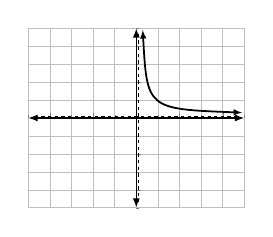
\begin{tikzpicture}[scale=\gridscale]
\begin{axis}[\axisfive]

\draw[<->, >=latex, ultra thick](0.3,4.9)..controls(0.5,0.5) ..(4.9,0.3);
\draw[thin, dashed](-4.7,0.1)--(4.7,0.1);
\draw[thin, dashed](0.1,4.7)--(0.1,-4.7); 

\end{axis} 
\end{tikzpicture}  
%6
\item \input{\figdir/fig-domain-and-range-of-a-function-b6} 
\end{multicols} 
\end{enumerate}  

B. Find the domain of each function.
\begin{enumerate}[label = \arabic*. ]
\item \hspce ${g(x)  = x-7 }$ 
\vspce 
\item \hspce ${g(x)  =  \sqrt{x+1} }$ 
\vspce 
\item \hspce ${ g(x) = \displaystyle  \frac{3x+4}{x-1} }$ 
\vspce 
\item \hspce ${ g(x)  =  \sqrt{ 2x-4} }$ 
\vspce 
\item \hspce ${g(x)  = \displaystyle  \frac{x+4}{3x-5} }$ 
\end{enumerate}  

\end{frame}

% frame 3
\vertadjustb
\begin{frame} 
\begin{center}
\textbf{Domain and Range of a Function}
\end{center}

\vspace*{1ex}

Domain: the set of all permissible values of $x$ that  give real values  for  $y$ 
 
\vspce 

Range: the set of permissible  values  for ${y }$   or  ${f(x) }$  that give the values of  ${x }$   real numbers

\vspce 

Asymptote: a line that the graph of a function approaches but never intersects

 
\def\figdir{/storage/emulated/0/Documents/documents/latex/1920/Grade-8/2nd/domain-and-range-of-a-function/f}

\textbf{Practice Exercises}

\vspce

A. Determine the domain and the range of each graph.
\begin{enumerate}[label = \arabic*. ]
\begin{multicols}{2}
%1
\item 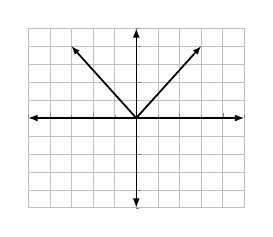
\begin{tikzpicture}[scale=\gridscale]
\begin{axis}[\axisfive]

\draw[->, >=latex, ultra thick] (0,0) -- (-3,4);
\draw[->, >=latex, ultra thick] (0,0) -- (3,4);

\end{axis} 
\end{tikzpicture}  
%2
\item 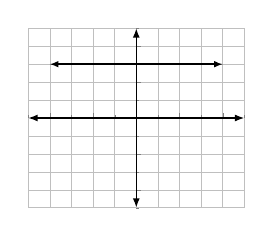
\begin{tikzpicture}[scale=\gridscale]
\begin{axis}[\axisfive]

\draw[<->, >=latex, ultra thick] (-4,3) -- (4,3);

\end{axis} 
\end{tikzpicture}  
%3
\item 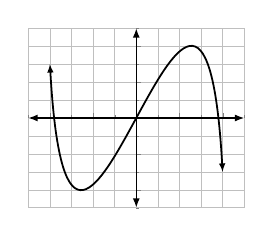
\begin{tikzpicture}[scale=\gridscale]
\begin{axis}[\axisfive]

\draw[<->, >=latex, ultra thick](-4,3)..controls(-3,-18) and (3,18)..(4,-3);

\end{axis} 
\end{tikzpicture}  
%4
\item 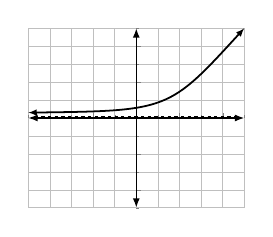
\begin{tikzpicture}[scale=\gridscale]
\begin{axis}[\axisfive]

\draw[<->, >=latex, ultra thick](-5,0.3)..controls(1.5,0.4) ..(5,5);
\draw[thin, dashed](-4.7,0.1)--(4.7,0.1); 

\end{axis} 
\end{tikzpicture}  
%5 
\item 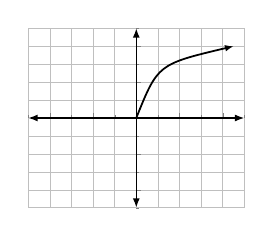
\begin{tikzpicture}[scale=\gridscale]
\begin{axis}[\axisfive]

\draw[->, >=latex, ultra thick](0,0.)..controls(1,3) ..(4.5,4);

\end{axis} 
\end{tikzpicture}  
%6
\item 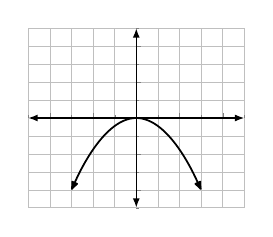
\begin{tikzpicture}[scale=\gridscale]
\begin{axis}[\axisfive]

\draw[<->, >={Latex[round]},  ultra thick] (-3,-4) parabola bend (0,0) (3,-4);

\end{axis} 
\end{tikzpicture}  
\end{multicols} 
\end{enumerate}  
B. Find the domain of each function.
\begin{enumerate}[label = \arabic*. ]
\item \hspce ${g(x)  = 5x+1 }$ 
\vspce 
\item \hspce ${g(x)  =  \sqrt{x} }$ 
\vspce 
\item \hspce ${ g(x) = \displaystyle  \frac{x+4}{x-2} }$ 
\vspce 
\item \hspce ${ g(x)  =  \sqrt{ x-8}}$ 
\vspce 
\item \hspce ${g(x)  =  \displaystyle  \frac{3x}{x+6}}$ 
\end{enumerate}  
%\def\figdir{/storage/emulated/0/Documents/documents/latex/1920/Grade-8/2nd/domain-and-range-of-a-function/f}

\textbf{Problem Set}

\vspce

A. Determine the domain and the range of each graph.
\begin{enumerate}[label = \arabic*. ]
\begin{multicols}{2}
%1
\item 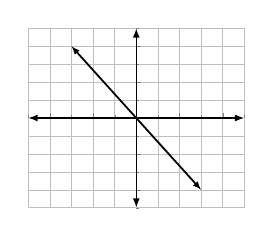
\begin{tikzpicture}[scale=\gridscale]
\begin{axis}[\axisfive]

\draw[<->, >=latex, ultra thick] (-3,4) -- (3,-4);

\end{axis} 
\end{tikzpicture}  
%2
\item 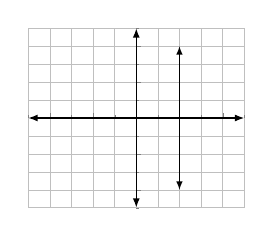
\begin{tikzpicture}[scale=\gridscale]
\begin{axis}[\axisfive]

\draw[<->, >=latex, ultra thick] (2,4) -- (2,-4);

\end{axis} 
\end{tikzpicture}  
%3
\item 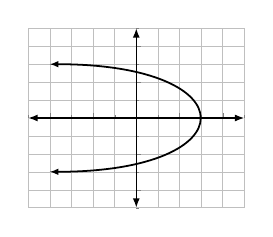
\begin{tikzpicture}[scale=\gridscale]
\begin{axis}[\axisfive]

\draw[<->, >=latex, ultra thick](-4,3)..controls(5.2,3) and (5.2,-3)..(-4,-3);

\end{axis} 
\end{tikzpicture}  
%4
\item 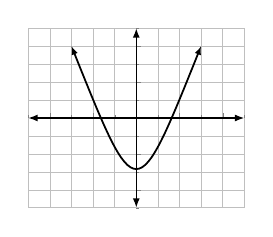
\begin{tikzpicture}[scale=\gridscale]
\begin{axis}[\axisfive]

\draw[<->, >=latex, ultra thick](-3,4)..controls(0,-5)..(3,4);

\end{axis} 
\end{tikzpicture}  
%5 
\item 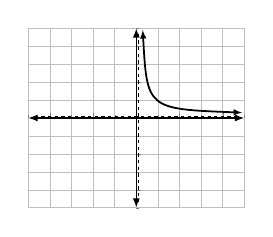
\begin{tikzpicture}[scale=\gridscale]
\begin{axis}[\axisfive]

\draw[<->, >=latex, ultra thick](0.3,4.9)..controls(0.5,0.5) ..(4.9,0.3);
\draw[thin, dashed](-4.7,0.1)--(4.7,0.1);
\draw[thin, dashed](0.1,4.7)--(0.1,-4.7); 

\end{axis} 
\end{tikzpicture}  
%6
\item \input{\figdir/fig-domain-and-range-of-a-function-b6} 
\end{multicols} 
\end{enumerate}  

B. Find the domain of each function.
\begin{enumerate}[label = \arabic*. ]
\item \hspce ${g(x)  = x-7 }$ 
\vspce 
\item \hspce ${g(x)  =  \sqrt{x+1} }$ 
\vspce 
\item \hspce ${ g(x) = \displaystyle  \frac{3x+4}{x-1} }$ 
\vspce 
\item \hspce ${ g(x)  =  \sqrt{ 2x-4} }$ 
\vspce 
\item \hspce ${g(x)  = \displaystyle  \frac{x+4}{3x-5} }$ 
\end{enumerate}  

\end{frame}

% frame 4
\vertadjustb
\begin{frame} 
%\begin{center}
\textbf{Domain and Range of a Function}
\end{center}

\vspace*{1ex}

Domain: the set of all permissible values of $x$ that  give real values  for  $y$ 
 
\vspce 

Range: the set of permissible  values  for ${y }$   or  ${f(x) }$  that give the values of  ${x }$   real numbers

\vspce 

Asymptote: a line that the graph of a function approaches but never intersects


%\def\figdir{/storage/emulated/0/Documents/documents/latex/1920/Grade-8/2nd/domain-and-range-of-a-function/f}

\textbf{Practice Exercises}

\vspce

A. Determine the domain and the range of each graph.
\begin{enumerate}[label = \arabic*. ]
\begin{multicols}{2}
%1
\item 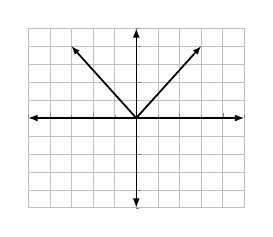
\begin{tikzpicture}[scale=\gridscale]
\begin{axis}[\axisfive]

\draw[->, >=latex, ultra thick] (0,0) -- (-3,4);
\draw[->, >=latex, ultra thick] (0,0) -- (3,4);

\end{axis} 
\end{tikzpicture}  
%2
\item 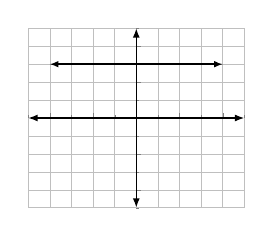
\begin{tikzpicture}[scale=\gridscale]
\begin{axis}[\axisfive]

\draw[<->, >=latex, ultra thick] (-4,3) -- (4,3);

\end{axis} 
\end{tikzpicture}  
%3
\item 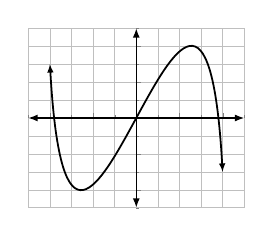
\begin{tikzpicture}[scale=\gridscale]
\begin{axis}[\axisfive]

\draw[<->, >=latex, ultra thick](-4,3)..controls(-3,-18) and (3,18)..(4,-3);

\end{axis} 
\end{tikzpicture}  
%4
\item 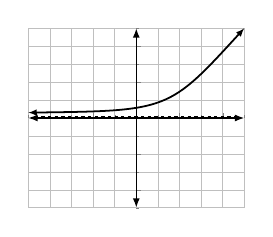
\begin{tikzpicture}[scale=\gridscale]
\begin{axis}[\axisfive]

\draw[<->, >=latex, ultra thick](-5,0.3)..controls(1.5,0.4) ..(5,5);
\draw[thin, dashed](-4.7,0.1)--(4.7,0.1); 

\end{axis} 
\end{tikzpicture}  
%5 
\item 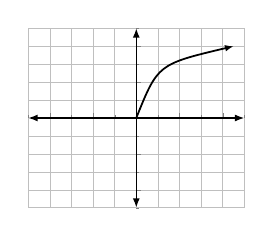
\begin{tikzpicture}[scale=\gridscale]
\begin{axis}[\axisfive]

\draw[->, >=latex, ultra thick](0,0.)..controls(1,3) ..(4.5,4);

\end{axis} 
\end{tikzpicture}  
%6
\item 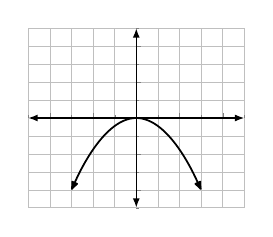
\begin{tikzpicture}[scale=\gridscale]
\begin{axis}[\axisfive]

\draw[<->, >={Latex[round]},  ultra thick] (-3,-4) parabola bend (0,0) (3,-4);

\end{axis} 
\end{tikzpicture}  
\end{multicols} 
\end{enumerate}  
%B. Find the domain of each function.
\begin{enumerate}[label = \arabic*. ]
\item \hspce ${g(x)  = 5x+1 }$ 
\vspce 
\item \hspce ${g(x)  =  \sqrt{x} }$ 
\vspce 
\item \hspce ${ g(x) = \displaystyle  \frac{x+4}{x-2} }$ 
\vspce 
\item \hspce ${ g(x)  =  \sqrt{ x-8}}$ 
\vspce 
\item \hspce ${g(x)  =  \displaystyle  \frac{3x}{x+6}}$ 
\end{enumerate}  
%\input{hand-domain-and-range-of-a-function-input2}
\vspace*{1ex}
\def\figdir{/storage/emulated/0/Documents/documents/latex/1920/Grade-8/2nd/domain-and-range-of-a-function/f}

\textbf{Problem Set}

\vspce

A. Determine the domain and the range of each graph.
\begin{enumerate}[label = \arabic*. ]
\begin{multicols}{2}
%1
\item 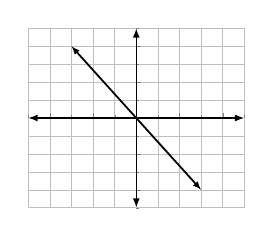
\begin{tikzpicture}[scale=\gridscale]
\begin{axis}[\axisfive]

\draw[<->, >=latex, ultra thick] (-3,4) -- (3,-4);

\end{axis} 
\end{tikzpicture}  
%2
\item 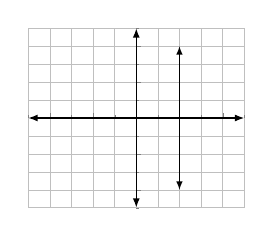
\begin{tikzpicture}[scale=\gridscale]
\begin{axis}[\axisfive]

\draw[<->, >=latex, ultra thick] (2,4) -- (2,-4);

\end{axis} 
\end{tikzpicture}  
%3
\item 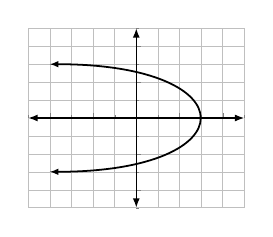
\begin{tikzpicture}[scale=\gridscale]
\begin{axis}[\axisfive]

\draw[<->, >=latex, ultra thick](-4,3)..controls(5.2,3) and (5.2,-3)..(-4,-3);

\end{axis} 
\end{tikzpicture}  
%4
\item 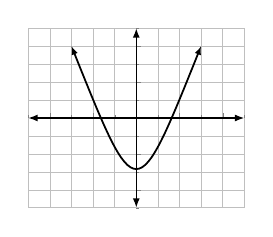
\begin{tikzpicture}[scale=\gridscale]
\begin{axis}[\axisfive]

\draw[<->, >=latex, ultra thick](-3,4)..controls(0,-5)..(3,4);

\end{axis} 
\end{tikzpicture}  
%5 
\item 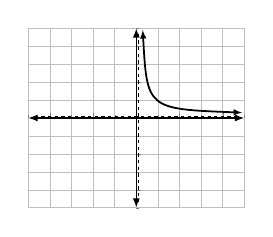
\begin{tikzpicture}[scale=\gridscale]
\begin{axis}[\axisfive]

\draw[<->, >=latex, ultra thick](0.3,4.9)..controls(0.5,0.5) ..(4.9,0.3);
\draw[thin, dashed](-4.7,0.1)--(4.7,0.1);
\draw[thin, dashed](0.1,4.7)--(0.1,-4.7); 

\end{axis} 
\end{tikzpicture}  
%6
\item \input{\figdir/fig-domain-and-range-of-a-function-b6} 
\end{multicols} 
\end{enumerate}  

B. Find the domain of each function.
\begin{enumerate}[label = \arabic*. ]
\item \hspce ${g(x)  = x-7 }$ 
\vspce 
\item \hspce ${g(x)  =  \sqrt{x+1} }$ 
\vspce 
\item \hspce ${ g(x) = \displaystyle  \frac{3x+4}{x-1} }$ 
\vspce 
\item \hspce ${ g(x)  =  \sqrt{ 2x-4} }$ 
\vspce 
\item \hspce ${g(x)  = \displaystyle  \frac{x+4}{3x-5} }$ 
\end{enumerate}  


\end{frame}

\end{document}

